\documentclass[11pt,letterpaper]{article}

% Compile from the template/ folder: latexmk -pdf -interaction=nonstopmode demo.tex
% This path mirrors how course main.tex files load the shared preamble.
% Shared formatting for course notes. Loaded by each course's main.tex.
\usepackage[T1]{fontenc}
\usepackage[utf8]{inputenc}
\usepackage{lmodern}
\linespread{1.15}
\usepackage[margin=1in]{geometry}
\usepackage{amsmath,amssymb,amsthm}
\usepackage{mathtools}
\usepackage{graphicx}
\usepackage{booktabs}
\usepackage{enumitem}
\usepackage{xcolor}
\usepackage{hyperref}
\usepackage{tikz}
\usetikzlibrary{decorations.pathreplacing,positioning}
\usepackage{xparse}
\usepackage{etoolbox}

\hypersetup{colorlinks=true,linkcolor=blue!50!black,urlcolor=blue!50!black}
\setlength{\parindent}{0pt}
\setlength{\parskip}{0.5em}
\setlist{nosep}

% Unnumbered section headings: entries show as "Week 1", not "1 Week 1",
% both in the body and in the table of contents.
\setcounter{secnumdepth}{0}

% Each \section (i.e. each week's entry) starts on its own new page. The
% \newpage that used to follow \tableofcontents in each course's main.tex
% is redundant now and has been removed, so week 1 isn't pushed to a blank
% page by this.
\pretocmd{\section}{\newpage}{}{\errmessage{Failed to patch \string\section}}

% Tracks whether \section was the most recent sectioning/lecture command,
% so a \newlecture immediately following a \section (the usual "week's
% first lecture" case) doesn't also throw in its own \newpage, which would
% otherwise leave a blank page between the two. Set true by \section, and
% cleared by \newlecture whether or not it was true, so it only fires for
% a \newlecture that directly follows a \section (nothing else in between).
\newbool{newlecture@justsection}
\pretocmd{\section}{\booltrue{newlecture@justsection}}{}{\errmessage{Failed to patch \string\section}}

% Custom head format: bold, unparenthesized title, with a \quad gap after
% the number (e.g. "Theorem 3.2  Distribution" instead of "Theorem 3.2
% (Distribution)."), reusing amsthm's usual spacing/punctuation otherwise.
% When a title is given, the body text starts on its own new line below the
% head instead of running inline after it; untitled (auto-numbered-only)
% instances stay inline as usual. Body text is upright (not italic) for all
% six environments. Two variants share this head format but differ in
% end-of-head punctuation: theorem/lemma/proposition/exercise keep a
% trailing period, definition/example drop it (no period after the title).
\makeatletter
\newcommand{\thmpunct}{.}
\newtheoremstyle{boldhead}{}{}{\normalfont}{}{\bfseries}{\thmpunct}{5pt plus 1pt minus 1pt}%
    {\thmname{#1}\thmnumber{\@ifnotempty{#1}{ }#2}\thmnote{\@ifnotempty{#3}{\quad#3}}%
     \@ifnotempty{#3}{\def\thmheadnl{\newline}\thm@headsep\z@skip}{}}
\newtheoremstyle{boldheadnp}{}{}{\normalfont}{}{\bfseries}{}{5pt plus 1pt minus 1pt}%
    {\thmname{#1}\thmnumber{\@ifnotempty{#1}{ }#2}\thmnote{\@ifnotempty{#3}{\quad#3}}%
     \@ifnotempty{#3}{\def\thmheadnl{\newline}\thm@headsep\z@skip}{}}
\makeatother

\theoremstyle{boldhead}
\newtheorem{theorem}{Theorem}
\newtheorem{lemma}[theorem]{Lemma}
\newtheorem{proposition}[theorem]{Proposition}
\newtheorem{corollary}[theorem]{Corollary}
\newtheorem{exercise}[theorem]{Exercise}
\theoremstyle{boldheadnp}
\newtheorem{definition}[theorem]{Def.}
\newtheorem{example}[theorem]{Example}
\theoremstyle{remark}
\newtheorem*{remark}{Remark}

% \begin{theorem}[Title][2.7]: both optional arguments are new on top of
% the environments' usual single bracket. The first argument still behaves
% exactly like plain amsthm's optional title (existing notes using
% \begin{example}[Some Name] etc. are unaffected). The second argument, if
% given, overrides the displayed number (e.g. to match a textbook's own
% numbering) instead of the shared theorem counter's automatic value; the
% counter itself still advances normally, so later auto-numbered
% environments are unaffected too.
\newcommand{\addtitleandnumber}[1]{%
    \csletcs{#1orig}{#1}%
    \csletcs{end#1orig}{end#1}%
    \RenewDocumentEnvironment{#1}{o o}{%
        \IfValueT{##2}{\ifblank{##2}{}{\renewcommand{\thetheorem}{##2}}}%
        \IfValueTF{##1}{\ifblank{##1}{\csname#1orig\endcsname}{\csname#1orig\endcsname[##1]}}{\csname#1orig\endcsname}%
    }{\csname end#1orig\endcsname}%
}
\addtitleandnumber{theorem}
\addtitleandnumber{lemma}
\addtitleandnumber{proposition}
\addtitleandnumber{corollary}
\addtitleandnumber{definition}
\addtitleandnumber{example}
\addtitleandnumber{exercise}

% Common mathematical notation.
\newcommand{\R}{\mathbb{R}}
\newcommand{\N}{\mathbb{N}}
\newcommand{\Z}{\mathbb{Z}}
\newcommand{\E}{\mathbb{E}}
\newcommand{\Prob}{\mathbb{P}}
\DeclareMathOperator{\Var}{Var}
\DeclareMathOperator{\Cov}{Cov}

% \newlecture[title][date]: bold, centered marker for the start of a new
% lecture. Both arguments are optional. Numbering runs continuously across
% the whole document (i.e. across all weeks' entries, not reset per
% \section), so the Nth \newlecture in the course is always "Lecture N".
% Each lecture starts on its own new page, except when it directly follows
% a \section heading (which already started a new page of its own), so the
% two stay together instead of leaving a blank page in between.
\newcounter{lecture}
\renewcommand{\thelecture}{\arabic{lecture}}
\NewDocumentCommand{\newlecture}{o o}{%
    \stepcounter{lecture}%
    \ifbool{newlecture@justsection}{}{\newpage}%
    \boolfalse{newlecture@justsection}%
    \par\vspace{1em}
    \begin{center}
        \textbf{\Large Lecture \thelecture\IfValueT{#1}{: #1}}\\[2pt]
        \IfValueT{#2}{\normalsize #2}
    \end{center}
    \vspace{0.5em}%
}

% Handwritten-note-style helpers: red definition labels, blue margin
% annotations, yellow highlights, underlined mini-headers.
\newcommand{\deflabel}[2]{\par\noindent{\color{red!70!black}\textbf{Def #1}}\quad\textbf{#2}\par\nobreak}
\newcommand{\exlabel}[2]{\par\noindent\textbf{Example #1}\quad\textbf{#2}\par\nobreak}
\newcommand{\heading}[1]{\par\noindent{\color{red!70!black}\textbf{#1}}\par}
\newcommand{\header}[1]{\par\vspace{0.5em}\noindent\textbf{#1}\par\vspace{-0.2em}}
\newcommand{\aside}[1]{\ifmmode{\color{blue!55!black}\text{\itshape #1}}\else{\color{blue!55!black}\itshape #1}\fi}
\newcommand{\hly}[1]{\colorbox{yellow!55}{$#1$}}
\newcommand{\hlt}[1]{\colorbox{yellow!55}{#1}}
% \boldmath makes any math the argument switches into (e.g. \rb{$r$}) use
% the bold math version automatically, so callers don't need to manually
% wrap math content in \boldsymbol{}.
\newcommand{\rb}[1]{{\color{red!70!black}\boldmath\textbf{#1}}}
\renewcommand{\b}[1]{\textbf{#1}}
\definecolor{navy}{RGB}{0,0,128}
\newcommand{\dbb}[1]{{\color{navy}\textbf{#1}}}
\newcommand{\db}[1]{{\color{navy}#1}}


\title{Course Notes Template --- Feature Demo\\[0.5em]\large Every environment and shortcut, shown with its source}
\author{Reference document, not a real course}
\date{}

\begin{document}
\maketitle
\tableofcontents
\newpage

\section{What this file is}
This is a reference build, not a lecture entry. Each section below pairs the
\texttt{verbatim} source for one template feature with what it actually
renders to, so you can copy the pattern you need straight into an entry file.

\section{Math shortcuts}
Defined in \texttt{preamble.tex} so you never have to type \texttt{\textbackslash mathbb\{R\}} by hand.

\begin{verbatim}
\R, \N, \Z, \E, \Prob \quad \Var(X), \Cov(X,Y)
\end{verbatim}
Renders as: $\R,\ \N,\ \Z,\ \E,\ \Prob \quad \Var(X),\ \Cov(X,Y)$

\section{Theorem-style environments}
\texttt{theorem}, \texttt{lemma}, and \texttt{proposition} share one counter
and use bold-header, italic-body plain style. The bracketed name is optional.

\begin{verbatim}
\begin{theorem}[Complement rule]
  For any event $A$, $\Prob(A^c) = 1 - \Prob(A)$.
\end{theorem}
\end{verbatim}
Renders as:
\begin{theorem}[Complement rule]
  For any event $A$, $\Prob(A^c) = 1 - \Prob(A)$.
\end{theorem}

\begin{verbatim}
\begin{lemma}
  Every convergent sequence is bounded.
\end{lemma}

\begin{proposition}
  The empty set is a subset of every set.
\end{proposition}
\end{verbatim}
Renders as:
\begin{lemma}
  Every convergent sequence is bounded.
\end{lemma}
\begin{proposition}
  The empty set is a subset of every set.
\end{proposition}

\section{Definition-style environments}
\texttt{definition}, \texttt{example}, and \texttt{exercise} use upright body
text and share the same counter sequence as the theorem-style set above.

\begin{verbatim}
\begin{definition}[Independence]
  Events $A$ and $B$ are independent if
  $\Prob(A \cap B) = \Prob(A)\Prob(B)$.
\end{definition}
\end{verbatim}
Renders as:
\begin{definition}[Independence]
  Events $A$ and $B$ are independent if
  $\Prob(A \cap B) = \Prob(A)\Prob(B)$.
\end{definition}

\begin{verbatim}
\begin{example}
  Rolling a fair die: $\Prob(\{1,3,5\}) = \tfrac{1}{2}$.
\end{example}

\begin{exercise}
  Show that $\Prob(A \cup B) = \Prob(A) + \Prob(B) - \Prob(A \cap B)$.
\end{exercise}
\end{verbatim}
Renders as:
\begin{example}
  Rolling a fair die: $\Prob(\{1,3,5\}) = \tfrac{1}{2}$.
\end{example}
\begin{exercise}
  Show that $\Prob(A \cup B) = \Prob(A) + \Prob(B) - \Prob(A \cap B)$.
\end{exercise}

\section{Remarks and proofs}
\texttt{remark} is unnumbered. \texttt{proof} comes from \texttt{amsthm}
automatically and ends with the usual tombstone.

\begin{verbatim}
\begin{remark}
  Independence is a modelling assumption, not something you can see
  directly in raw data.
\end{remark}

\begin{proof}
  Immediate from $\Prob(A) + \Prob(A^c) = 1$.
\end{proof}
\end{verbatim}
Renders as:
\begin{remark}
  Independence is a modelling assumption, not something you can see
  directly in raw data.
\end{remark}
\begin{proof}
  Immediate from $\Prob(A) + \Prob(A^c) = 1$.
\end{proof}

\section{Cross-references}
Attach a \texttt{\textbackslash label} to any numbered environment and refer
back to it with \texttt{\textbackslash ref}.

\begin{verbatim}
\begin{theorem}[Bayes' rule]\label{thm:bayes}
  $\Prob(A\mid B) = \dfrac{\Prob(B\mid A)\Prob(A)}{\Prob(B)}$.
\end{theorem}

See Theorem~\ref{thm:bayes} above.
\end{verbatim}
Renders as:
\begin{theorem}[Bayes' rule]\label{thm:bayes}
  $\Prob(A\mid B) = \dfrac{\Prob(B\mid A)\Prob(A)}{\Prob(B)}$.
\end{theorem}
See Theorem~\ref{thm:bayes} above.

\section{Handwritten-note formatting helpers}
These extra commands (also in \texttt{preamble.tex}) reproduce the look of
red definition labels, blue margin comments, and yellow highlights from
scanned handwritten notes; see \texttt{STA347/entries/week01.tex} for a full
worked example.

\begin{verbatim}
\deflabel{2.1}{Conditional Probability}
\begin{quote}
  $\Prob(A\mid B) = \Prob(A\cap B)/\Prob(B)$ when $\Prob(B) > 0$.
\end{quote}
\aside{This is undefined if $B$ has probability zero.}

\heading{Key difference:}
Conditioning rescales the sample space; independence does not.

Uniform convergence needs \hly{a single threshold $N$} for every $x$.
\end{verbatim}
Renders as:

\deflabel{2.1}{Conditional Probability}
\begin{quote}
  $\Prob(A\mid B) = \Prob(A\cap B)/\Prob(B)$ when $\Prob(B) > 0$.
\end{quote}
\aside{This is undefined if $B$ has probability zero.}

\heading{Key difference:}
Conditioning rescales the sample space; independence does not.

Uniform convergence needs \hly{a single threshold $N$} for every $x$.

\section{Diagrams with TikZ}
\texttt{tikz} and the \texttt{decorations.pathreplacing} library are loaded
by the preamble, so any entry can draw a quick sketch inline.

\begin{verbatim}
\begin{center}
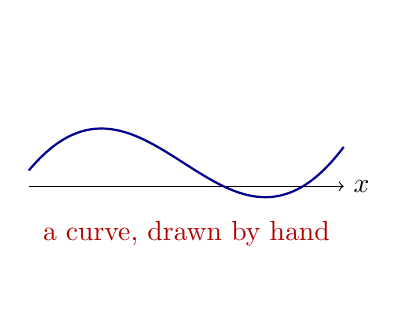
\begin{tikzpicture}
  \draw[->] (0,0) -- (4,0) node[right]{$x$};
  \draw[thick, blue!55!black] (0,0.2) .. controls (1.5,2) and (2.5,-1.5)
    .. (4,0.5);
  \node[red!70!black] at (2,-0.6) {a curve, drawn by hand};
\end{tikzpicture}
\end{center}
\end{verbatim}
Renders as:
\begin{center}
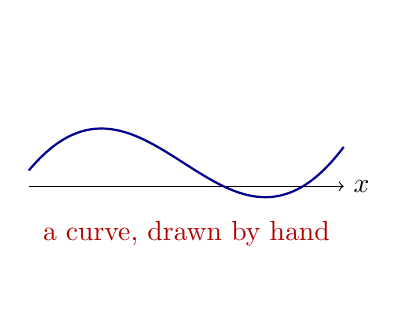
\begin{tikzpicture}
  \draw[->] (0,0) -- (4,0) node[right]{$x$};
  \draw[thick, blue!55!black] (0,0.2) .. controls (1.5,2) and (2.5,-1.5)
    .. (4,0.5);
  \node[red!70!black] at (2,-0.6) {a curve, drawn by hand};
\end{tikzpicture}
\end{center}

\section{Lists}
\texttt{enumitem} is loaded with \texttt{nosep}, so list items sit close
together the way handwritten bullet points do.

\begin{verbatim}
\begin{itemize}
  \item Sample space $\Omega$
  \item Event space $\mathcal{F}$
  \item Probability measure $\Prob$
\end{itemize}
\end{verbatim}
Renders as:
\begin{itemize}
  \item Sample space $\Omega$
  \item Event space $\mathcal{F}$
  \item Probability measure $\Prob$
\end{itemize}

\section{Tables}
\texttt{booktabs} gives the clean horizontal-rule table style (no vertical
rules).

\begin{verbatim}
\begin{center}
\begin{tabular}{lcc}
  \toprule
  Distribution & Mean & Variance \\
  \midrule
  $\text{Bernoulli}(p)$ & $p$ & $p(1-p)$ \\
  $\text{Poisson}(\lambda)$ & $\lambda$ & $\lambda$ \\
  \bottomrule
\end{tabular}
\end{center}
\end{verbatim}
Renders as:
\begin{center}
\begin{tabular}{lcc}
  \toprule
  Distribution & Mean & Variance \\
  \midrule
  $\text{Bernoulli}(p)$ & $p$ & $p(1-p)$ \\
  $\text{Poisson}(\lambda)$ & $\lambda$ & $\lambda$ \\
  \bottomrule
\end{tabular}
\end{center}

\section{Links}
\texttt{hyperref} is loaded with colored links, so both cross-references
(Section~\ref{sec:links}) and external URLs render in color automatically.
\label{sec:links}

\begin{verbatim}
See \href{https://www.overleaf.com}{Overleaf} for an online editor.
\end{verbatim}
Renders as: See \href{https://www.overleaf.com}{Overleaf} for an online editor.

\section{Images}
\texttt{graphicx} is loaded but no image ships with this demo, so the call
below is shown only as source --- point it at a real file in a course-local
\texttt{figures/} folder to use it.

\begin{verbatim}
\includegraphics[width=0.6\textwidth]{figures/diagram.png}
\end{verbatim}

\end{document}
